\def\year{2019}\relax
%File: formatting-instruction.tex
\documentclass[letterpaper]{article} %DO NOT CHANGE THIS
\usepackage{aaai19}  %Required
\usepackage{times}  %Required
\usepackage{helvet}  %Required
\usepackage{courier}  %Required
\usepackage{url}  %Required
\usepackage{graphicx}  %Required
\frenchspacing  %Required
\setlength{\pdfpagewidth}{8.5in}  %Required
\setlength{\pdfpageheight}{11in}  %Required
\newcommand{\C}{\ensuremath{C}}
\newcommand{\N}{\mbox{$I\!\!N$}}
\newtheorem{definition}{Definition}
\newtheorem{example}{Example}
\newtheorem{proposition}{Proposition}
\newtheorem{proof}{Proof}
%PDF Info Is Required:
  \pdfinfo{
/Title (Argumentation-Based Representation and Explanation of Value Driven Agent)
/Author (Beishui Liao et al.)}
\setcounter{secnumdepth}{0}  
 \begin{document}
% The file aaai.sty is the style file for AAAI Press 
% proceedings, working notes, and technical reports.
%
\title{Representation, Justification and Explanation in a Value Driven Agent: An Argumentation-Based Approach}

\author{%Beishui Liao \\ 
%Zhejiang University \\Hangzhou, China\\
%baiseliao@zju.edu.cn\And 
\#1 author\\
Artificial Intelligence; Logic \\
 \And
 \#2 author\\
Artificial Intelligence \\
 \And
 \#3 author\\
Philosophy; Applied Ethics
%Michael Anderson \\ University of Hartford \\ Hartford, CT, USA \\ anderson@hartford.edu
%\And Susan Leigh Anderson \\ University of Connecticut \\ Storrs, CT, USA \\ susan.anderson@uconn.edu
%\And Leendert van der Torre\\University of Luxembourg\\Luxembourg\\leon.vandertorre@uni.lu
}

\maketitle
\begin{abstract}
For an autonomous system, the ability to justify and explain its decision making is crucial to improve its transparency and trustworthiness. This paper proposes an argumentation-based approach to represent, justify and explain the decision making of a value driven agent (VDA). By using a newly defined formal language, some implicit knowledge of a VDA is made explicit. The selection of an action in each situation is justified by constructing and comparing arguments supporting different actions. In terms of a constructed argumentation framework and its extensions, the reasons for explaining an action are defined in terms of the arguments for or against the action, by exploiting their defeat relation, as well as their premises and conclusions.  

%Research questions:  1) how to obtain and represent human values for the purpose of value alignment? 2) how to apply these values in the ethical decision-making of an agent? 3) how to explain the agent's actions? 

%Our solution: i) KR approach:  knowledge - norms, ethical values and preferences over norms and actions; ii) decision-making and explanation by exploiting argumentation; iii) verification or justification: aligning to human values through ethicists and aligning to norms; explanation: why an action is not taken - in terms of attack relation, values, and norms that are applied,  why an action is taken - in terms of support and defense relation, values and norms that are applied. 
\end{abstract}

\section{Introduction}
To improve the transparency and trustworthiness of autonomous systems, different approaches have been proposed to provide explanations for such systems, see, e.g., \cite{Cocarascu2018,DBLP:conf/ijcai/ShihCD18,DBLP:journals/corr/abs-1806-08055}. Working along these lines, we introduce an approach for representing, justifying and explaining the decision making of a value driven agent, or VDA for short \cite{DBLP:conf/aaai/AndersonAB17}.  

We define a VDA as an autonomous agent that decides its next action using an ethical preference relation over actions, termed a \textit{principle}, that is abstracted from a set of cases using machine learning. This \textit{case-supported, principle based approach} (CPB) uses a representation scheme that includes \textit{ethically relevant features} (e.g. harm, good, etc.) and their incumbent duties to either minimize or maximize them (e.g. minimize harm, maximize good), \textit{actions} characterized by integer degrees of presence or absence of ethically relevant features (and so, indirectly, the duties it satisfies or violates), and \textit{cases} comprised of the differences of the corresponding duty satisfaction/violation degrees of two actions.  	

A principle of ethical preference is defined as a disjunctive normal form predicate in terms of lower bounds for duty differentials of a case: 
[place logical representation of principle here]
where $\Delta d_i$ denotes the difference of a corresponding values of duty \textit{i} in actions$\ a_1$ and$\ a_2$ (the actions of the case in question) and$\ v_i,_j$ denotes the lower bound of duty \textit{i} in disjunct \textit{j} such that$\ p(a_1,a_2)$ returns \textit{true} if action$\ a_1$  is ethically preferable to action$\ a_2$.  

\textit{Inductive logic programming} (ILP) techniques are used to abstract principles from judgments of the ethicists on specific cases where a consensus exists as to the ethically relevant features involved, the relative levels of satisfaction or violation of their correlative duties, and the action that is considered ethically preferable.  Resulting from this process is a set of sets of lower bounds for which principle$\ p$ will return \textit{true} for all positive cases presented to it (i.e. where the first action is ethically preferable to the second) and \textit{false} for all negative cases (i.e. where the first action is \textit{not} ethically preferable to the second). That is, for every positive case, there is a clause of the principle that is true for the differential of the actions of the case and, for every negative case, no clause of the principle returns true for the differential of the actions of the case.  The principle is thus complete and consistent with respect to its training cases.  Further, given the nature of ILP, the lower bounds of the principle are sufficiently relaxed to cover cases other than those used in its training.

To use this principle to determine a VDA's next action, it is necessary to associate each of the VDA's possible actions with a vector of values representing levels of satisfaction or violation of duties that that action exhibits in the current context. These duties either maximize or minimize ethically relevant features such as honoring commitments, maintaining readiness, harming the patient, etc.   The current context is represented as a set of Boolean perceptions determined from initial input and sensor data. These values are determined using a decision tree abstracted from examples of Boolean perceptions and their corresponding sets of duty satisfaction/violation values.  The decision making process of a VDA, then, is as follows:  sense the state of the world and abstract it into a set of Boolean perceptions, determine the vectors of duty satisfaction or violation of all actions with respect to this state by the decision tree, and sort the actions in order of ethical preference using the principle such that the first action in the sorted list is the most ethically preferable one.

It is interesting to note that in the VDA there are several kinds of knowledge that can be used for justification and explanation, including the relation between perceptions and actions determined by the decision tree, the ethical consequences of an action represented by a vector of duty satisfaction or violation values of the action,  disjuncts in the clause of the principle that are used to order two actions, and the cases from which these disjuncts are abstracted. However, this knowledge has not been explicitly represented and used for justification of actions or providing explanations. In this paper, we will address this problem by exploiting formal argumentation. 
The structure of this paper is as follows. Section 2 introduces a formalism for representing knowledge of a value driven agent. In Section 3, we present an argumentation-based justification and explanation approach. In section 4, we discuss some further research problems of justifying and explaining more sophisticated autonomous agents. Finally, we conclude the paper in Section 5. 


\section{Representing value driven agent}
In this section, we first introduce a formal language and then use it to represent the knowledge and the model of a VDA. 

%In a VDA, there are a set of perceptions used to reflect the state of the world, called a \emph{ situation} in this paper. By using a decision tree, an action matrix is produced with respect to the situation. The relation between a situation and an action matrix can be represented by a defeasible rule. Then, in each situation, the preference relation between various actions is defined in terms of a principle, which is learned  from a set of cases by using ILP.  Here, a principle is a set of vectors defining the lower bound of the differences between corresponding duties of any two actions. 

%Then, in each case, whether an action is ethically preferable is learned from a set of cases by using ILP.  

%In this section, we use a logical language to formalize the following nations: perceptions, actions, duties and principle. 
The language of a VDA is composed of literals, perceptions, actions and duties.


\begin{definition}[Language]
Let $\mathcal{L} = (L, P, A, D)$ be a language consisting of a set of literals $L$, a set of perceptions $P \subseteq L$, a set of actions $A$ and a set of duties $D$, where each literal is a propositional atom or the negation of an atom, and $L, A$ and $D$ are pairwise disjoint. For $l_1, l_2\in L$, we write $l_1 = - l_2$ just in case $l_1 = \neg l_2$ or $l_2 = \neg l_1$. 
\end{definition}

\begin{example}[Language]
In \cite{DBLP:journals/pieee/Anderson19}, there are 10 atoms of perceptions: low battery (lb), medication reminder time (mrt), reminded (r), refused medication (rm), fully charged (fc), no interaction (ni), warned (w), persistent immobility (pi), engaged (e), ignored waning (iw);  6 actions: charge, remind, engage, warn, notify and seek task; and 7 duties: maximize honor commitments ($\mathrm{MHC}$), maximize maintain readiness ($\mathrm{MMR}$), minimize harm to patient ($\mathrm{mH2P}$), maximize good to patient ($\mathrm{MG2P}$), minimize non-interaction ($\mathrm{mNI}$), maximize respect autonomy ($\mathrm{MRA}$) and maximize prevent persistent immobility ($\mathrm{MPPI}$).
%LOW\_BATTERY (lb), 
%MEDICATION\_REMINDER\_TIME (mt), 
%\item REMINDED (rd), REFUSED\_MEDICATION (rm), 
%\item FULLY\_CHARGED (fc), 
%NO\_INTERACTION (ni), 
%\item WARNED (wd), 
%PERSISTENT\_IMMOBILITY (pi), 
%\item ENGAGED (ed), 
%IGNORED\_WARNING (iw)
%\end{description}
%When we get  $[$`TRUE', `FALSE', `FALSE', `FALSE', `FALSE', `FALSE', `FALSE', `FALSE', `FALSE', `FALSE'$]$ 
%A possible state of the world is $S_1 = \{lb, \neg mrt, \neg r, \neg rm, \neg fc, \neg ni, \neg w, \neg pi, \neg e, \neg iw\}$.
\end{example}

In \cite{DBLP:journals/pieee/Anderson19}, $L = P$. The state of the world is represented by a set of perceptions, called a \emph{situation} in this paper. 

\begin{definition}[Situation]
A situation $S$ is a subset of $L$, denoting a state of the world. %A trained case is a case after training. 
The (infinite) set of situations is denoted as $SIT$. 
\end{definition}

\begin{example}[Situation]
An example of the state of the world: $S_1 = \{lb,  \neg mrt, \neg r, \neg rm, \neg fc$, $\neg ni$, $\neg w$, $\neg pi$, $\neg e$, $\neg iw\}$.
\end{example}

In each situation, the duty satisfaction/violation values for each action are determined by a decision tree using the perceptions of the situation as input. A set of vectors of duty satisfaction/violation values of all actions in a situation is called an \emph{action matrix}. 

\begin{definition}[Action matrix of a situation]
A duty satisfaction value is a positive integer, while a duty violation value is a negative integer. In addition, if a duty is neither satisfied nor violated by the action, then the value is zero. Given an action $\alpha\in A$ and a situation $S\in SIT$, a vector of duty satisfaction/violation values for $\alpha$, denoted as  $v_S(\alpha)$, is a vector $v_S(\alpha) = ( d_1: v_{S, \alpha}(d_1), \dots, d_n: v_{S, \alpha}(d_n)  )$ where $v_{S, \alpha}(d_i)$ is the satisfaction/violation value of $d_i\in D$. Then, an action matrix of a situation $S$ is defined as $M_S = \{v_S(\alpha) \mid \alpha\in A\}$. The set of action matrices of all situations $SIT$ is denoted as $M_{SIT} = \{M_S \mid S\in SIT\}$. 
\end{definition}

In this definition, a vector of duty satisfaction/violation values for each action will be used to define the ethical preference over actions, by considering the ethical consequences of the actions in a given situation. 

For brevity, when the order of duties is clear,  $v_S(\alpha) = ( d_1: v_{S, \alpha}(d_1), \dots, d_n: v_{S, \alpha}(d_n)  )$ is also written as $v_S(\alpha) = ( v_{S, \alpha}(d_1), \dots,  v_{S, \alpha}(d_n)  )$. 

\begin{example}[Action matrix of a situation]\label{ex-action-matrix}
%In (Anderson \& Anderson, 2017), there are 7 duties: maximal honor commitments ($\mathrm{MHC}$), maximal maintain readiness ($\mathrm{MMD}$), minimal harm to patient ($\mathrm{MH2P}$), maximal good to patient ($\mathrm{MG2P}$), minimal non-interaction ($\mathrm{MNI}$), maximal respect autonomy ($\mathrm{MRA}$) and maximal prevent persistent immobility ($\mathrm{MPPI}$). 
Given a state of the world $S_1$, according to \cite{DBLP:journals/pieee/Anderson19},  the action matrix of $S_1$ is $M_{S_1} = \{v_{S_1}(charge), v_{S_1}(remind), v_{S_1}(engage), v_{S_1}(warn)$, $v_{S_1}(notify), v_{S_1}(seekTask)\}$, where
\begin{description}
\item $v_{S_1}(charge) = (0, 2,  0, -1, 0, 0, 0)$,
\item $v_{S_1}(remind) = (-1, -2, 0, -1, 0, 0, 0)$,
\item $v_{S_1}(engage) = (0, -2, 0, -1, 0, 0, 0)$,
\item $v_{S_1}(warn) = (0, 0, 0, -1, 0, -1, 0)$,
\item $v_{S_1}(notify) = (0, 0, 0, -1, 0, -2, 0)$,
\item $v_{S_1}(seekTask) = (0, -1, 0, 1, 0, 0, 0)$.
\end{description}
The duties in each vector are $\mathrm{MHC}$, $\mathrm{MMR}$, $\mathrm{mH2P}$, $\mathrm{MG2P}$, $\mathrm{mNI}$, $\mathrm{MRA}$ and $\mathrm{MPPI}$ in order.
\end{example}

Given a situation and its corresponding action matrix, actions are sorted by a principle.  This principle is discovered by applying inductive logic programming (ILP) techniques to a set of cases.  Clauses of the principle specify lower bounds of the differentials between corresponding duties of any two actions that must be met or exceeded to satisfy the clause.

\begin{definition}[Principle]
A principle is defined as  $\pi = \{u_1, \dots, u_k\}$, where $u_i =  ( d_1: u_i(d_1), ..., d_n: u_i(d_n)  )$, where $d_j$ is a duty, and $u_i(d_j)$ is the acceptable lower bound of the differentials between corresponding duties of any two actions in $A$. 
\end{definition}

For brevity, when the order of duties is clear, in a principle the lower bound of the differentials between duties is also written as $u_i =  ( u_i(d_1), ...,  u_i(d_n))$. 

\begin{example}[Principle]
According to \cite{DBLP:journals/pieee/Anderson19}, we have
$\pi = \{u_1, \dots, u_{10}\}$ where 
\begin{description}
\item $u_1 = (-1, -4, -4, -2, -4, -4, 2)$,
\item $u_2 = (-1, -4, -4, -2, 0, 0, 1)$,
\item $u_3 = (0, -3, 0, -1, 0, 1, 0)$,
\item $u_4 = (0, -3, 0, 1, 0, 0, 0)$,
\item $u_5 = (0, -1, 0, 0, 0, 0, 0)$,
\item $u_6 = (0, -3, 0, -1, 1, -1, 0)$,
\item $u_7 = (-1, -4, 1, -2, -4, -4, 0)$,
\item $u_8 = (1, -3, 0, -2, -4, -4, 0)$,
\item $u_9 = (0, 3, 0, -2, 0, 0, 0)$,
\item $u_{10} = (-1, -4, 1, -1, -4, -4, -1)$.
\end{description}
These 10 elements in $\pi$ correspond to 10 disjuncts of the principle in  \cite{DBLP:journals/pieee/Anderson19}.
\end{example}

Given a principle and two vectors of duty satisfaction/violation values, we may define a notion of ethical preference over actions. 
Let $v_{S}(\alpha_1) = ( d_1: v_{S,\alpha_1}(d_1), \dots, d_n: v_{S, \alpha_1}(d_n))$ and $v_{S}(\alpha_2) = ( d_1: v_{S,\alpha_2}(d_1), \dots, d_n: v_{S, \alpha_2}(d_n))$ be vectors of duty satisfaction/violation values. In the following definitions, we use 
 $w = v_{S}(\alpha_1) - v_{S}(\alpha_2) = (d_1: w(d_1), \dots, d_n: w(d_n))$ to denote a vector of the differentials of $v_{S}(\alpha_1)$ and $v_{S}(\alpha_2)$, where $w(d_1) = v_{S,\alpha_1}(d_1) - v_{S,\alpha_2}(d_1)$, \dots, $w(d_n) = v_{S,\alpha_1}(d_n) - v_{S,\alpha_2}(d_n)$. 
 
 \begin{definition}[Ethical preference over actions]
 Given a principle $\pi$, a situation $S$, two actions $\alpha_1$ and $\alpha_2$, and $w$, the differentials of $v_{S}(\alpha_1)$ and $v_{S}(\alpha_2)$, we say that $\alpha_1$ is ethically preferable (or equal) to $\alpha_2$ with respect to some $u\in \pi$, written as $v_{S}(\alpha_1) \ge_u v_{S}(\alpha_2)$, if and only if  for each $d_i: w(d_i)$ in $w$ and $d_i: u(d_i)$ in $u$, it holds that $w(d_i) \ge  u(d_i)$.
\end{definition}

In this definition, we make explicit the disjuncts $(u)$ in the clause of the principle that are used to order two actions. 

Given two actions $\alpha_1$ and $\alpha_2$, there might be more than one clause of $\pi$, say $u_1, u_2\in \pi$, such that $v_{S}(\alpha_1) \ge_{u_1} v_{S}(\alpha_2)$ and $v_{S}(\alpha_1) \ge_{u_2} v_{S}(\alpha_2)$. In order to compare relations with respect to different clauses of a principle, we introduce a notion of the relevance of a clause to a vector of differentials of duty satisfaction/violation values of two actions in terms of their distance. The intuition is that the larger the distance, the lesser the relevance between them. 

\begin{definition}[Relevance of principle clause]
Let $u\in \pi$ be a clause, and $w$ be a vector of the differentials of duty satisfaction/violation values of two actions. The relevance of $u$ to $w$ is defined as the distance between $u$ and $w$, written as $d(u, w)$, such that $d(u, w) = \sqrt{(u(d_1)-w(d_1))^2+\dots+(u(d_n)-w(d_n))^2}$. 
\end{definition}

\begin{example}[Relevance of principle clause]
Consider the distance between $w_1 = v_{S_1}(charge)-v_{S_1}(remind) = (1, 4, 0$, $0, 0, 0, 0)$ and $u_5$, $u_8$ and $u_9$ respectively. 
\begin{itemize}
    \item $d(u_5, w_1) = \sqrt{26}$.
    \item $d(u_8, w_1) = \sqrt{85}$.
    \item $d(u_9, w_1) = \sqrt{6}$.
\end{itemize}
\end{example}

\begin{definition}[Ethical preference over actions - cont.]
We say that $\alpha_1$ is ethically preferable (or
equal) to $\alpha_2$ with respect to their most relevant clause $u\in \pi$ if and only if $v_{S}(\alpha_1) \ge_u v_{S}(\alpha_2)$ and there exists no $u^\prime\in \pi$ such that $v_{S}(\alpha_1) \ge_{u^\prime} v_{S}(\alpha_2)$ and $d(u^\prime, w) < d(u, w)$, where $w = v_{S}(\alpha_1) - v_{S}(\alpha_2)$.
\end{definition}

\begin{example}[Ethical preference over actions - cont.]
Consider the actions $charge$ and $remind$. For each $u\in\{u_5,u_8,u_9\}$, $v_{S}(charge) \ge_u v_{S}(remind)$. Among them, $u_9$ is the most relevant clause with respect to $w_1$. 
\end{example}

Based on the above notions, a value driven agent (VDA) is formally defined as follows.

\begin{definition}[Value driven agent]
A value driven agent is a tuple $Ag = (\mathcal{L}, SIT, M, \pi)$ where $\mathcal{L} = (L, P, A, D)$.  %We say that a value driven agent is complete if and only if for any new case $S$, it holds that $S\in SIT$. 
\end{definition}

In a VDA, given a situation and an action matrix, a set of solutions can be defined as follows.   

\begin{definition}[Solution] \label{def-solution}
Let $Ag = (\mathcal{L}, SIT, M, \pi)$ be a value driven agent. Given a situation $S\in SIT$ and an action matrix $M_S\in M$, a solution of $Ag$ with respect to $S$ is $\alpha : v_{S}(\alpha)$ if and only if there is an ordering over $A$ with respect to $\pi$ such that $\alpha$ is the first action in the sorted list.  The set of all solutions of $Ag$ with respect to $S$ is denoted as $sol(Ag, M_S, \pi) = \{\alpha : v_{S}(\alpha) \mid \alpha\in A$ such that $\alpha : v_{S}(\alpha)$ is a solution of $Ag$ w.r.t. $S\}$.
\end{definition}

According to Definition \ref{def-solution}, we directly have the following proposition. 

\begin{proposition}[The number of solutions]
Given $Ag = (\mathcal{L}, SIT, M, \pi)$, a situation $S\in SIT$ and an action matrix $M_S\in M$, there are $k$ solutions of $Ag$ if and only if there are $k$ different orderings of $A$ with respect to $\pi$ such that there are $k$ different actions in the head of the sorted lists. 
\end{proposition}

Now, let us make explicit other knowledge that is implicit in a VDA , i.e., the relation between a situation and an action with its duty satisfaction/violation values. This relation is implied by the decision tree. In this paper, it is represented as a defeasible rule, called an \emph{action rule}. 

\begin{definition}[Action rule]\label{def-act-rul}
%There are two kinds of rules. 
Let $Ag = (\mathcal{L}, SIT, M, \pi)$ be a VDA, where $\mathcal{L} = (L, P, A, D)$. 
An action rule of $Ag$ under a situation $S\in SIT$ is $R: p_1, \dots, p_n \Rightarrow \alpha: v_S(\alpha)$, where $R$ is a label of the rule, $p_i\in S$ is a perception, $\alpha\in A$ is an action, $v_S(\alpha)$ is a vector of the duty satisfaction/violation values of $\alpha$ in the situation $S$. % A preference rule is $s: (u\in P) \wedge (v(\alpha) - v(\beta)\ge u)  \rightarrow  v(\alpha) \succeq v(\beta)$.
\end{definition}

An action rule $R: p_1, \dots, p_n \Rightarrow \alpha: v_S(\alpha)$ can be read as if $p_1, \dots$, $p_n$ hold, then performing action $\alpha$ will presumably bring the ethical consequence $v_S(\alpha)$. The set of all action rules of $Ag$ under situation $S$ is denoted as $RUL_S(Ag)$. Action rules can be automatically and dynamically generated and updated according to the data from a VDA. 


For convenience, $p_1, \dots, p_n$ in $R: p_1, \dots, p_n \Rightarrow \alpha: v_S(\alpha)$ is also written as $p_1 \wedge \dots \wedge p_n$.
%For brevity, when the context is clear, we omitted the literals that are not atoms within a rule. 

\begin{example}[Action rule] \label{ex-1}
Continuing Example \ref{ex-action-matrix}. Given 
$S_1$, there are six defeasible rules, where $LB = lb \wedge \neg mrt \wedge \neg r \wedge \neg rm \wedge \neg fc \wedge \neg ni$ $\wedge$ $\neg w \wedge \neg pi \wedge \neg e \wedge \neg iw$.
\begin{description}
\item $R_1: LB \Rightarrow  charge: v_{S_1}(charge)$. 
\item $R_2: LB \Rightarrow  remind: v_{S_1}(remind)$.
\item $R_3: LB \Rightarrow  engage: v_{S_1}(engage)$. 
\item $R_4: LB \Rightarrow  warn: v_{S_1}(warn)$.
\item $R_5: LB \Rightarrow  notify: v_{S_1}(notify)$. 
\item $R_6: LB \Rightarrow  seekTask: v_{S_1}(seekTask)$.
 \end{description}
% \begin{figure}[h!]
%  \centering
% 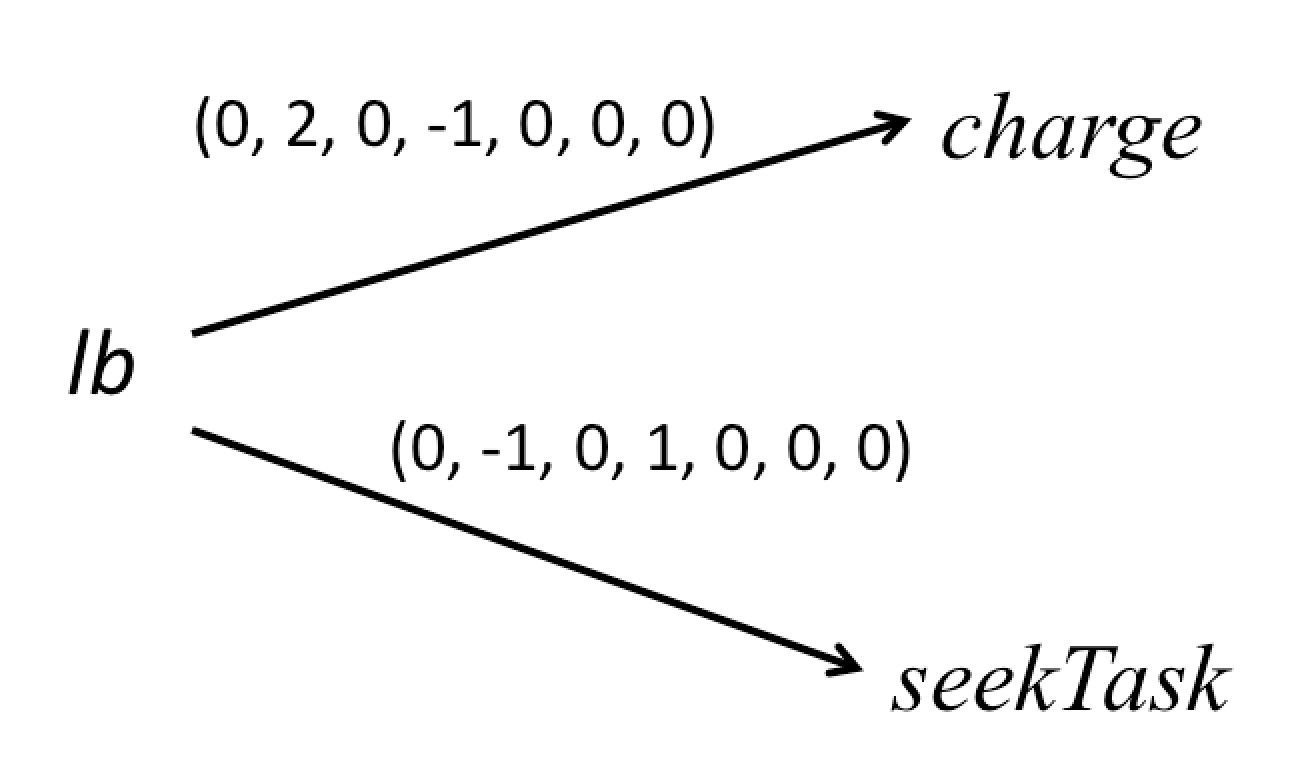
\includegraphics[width=0.3\textwidth]{exam1.png}
 % \caption{An example of rules in a situation}
%    \label{fig:ex-1}
%\end{figure}
\end{example}

Note that in this example, it is possible for an action to not satisfy any duties and there might be no effect on the conclusion of decision making if one removes those rules associated with them. However, theoretically, we have not ruled out the possibility that \textit{no} action satisfies \textit{any} duty in some situations, where the most preferable action would then be the one that violated duties the least. So, we remove nothing, keeping all rules constructed in terms of Definition \ref{def-act-rul}. 

In summarizing this section, we may conclude that the formal model of a VDA and the set of action rules properly capture the underlying knowledge of the VDA. In next section, we will introduce an argumentation-based approach for the justification and explanation of the decision-making a VDA. 

\section{Argumentation-based justification and explanation}
Argumentation in artificial intelligence is a formalism for representing and reasoning with inconsistent and incomplete information \cite{DBLP:journals/ai/Dung95}. It also provides various ways for explaining why a claim or a decision is made, in terms of justification, dialogue, and dispute trees \cite{DBLP:conf/comma/CyrasST16}, etc. In this section, we show how to justify and explain decision making of a VDA by using argumentation. 

In terms of structured argumentation (e.g., ASPIC$^+$ \cite{DBLP:journals/argcom/ModgilP14}), there are three basic notions including arguments, relations between arguments and argumentation semantics. We will define them in the setting of this paper. First, an argument is a set of reasons supporting a claim or an action. In what follows, for a given argument, the function $concl$ returns its conclusion, and $sub$ returns all its sub-arguments.
\begin{definition}[Argument]\label{def-arg}
%Let $Y = \{u^{\alpha\beta}  \mid \alpha, \beta\in A, u\in P: v(\alpha)-v(\beta)\ge u\}$.
Let $Ag = (\mathcal{L},  SIT, M, \pi)$ be a value driven agent, where $\mathcal{L} = (L, P, A, D)$. 
Argument $X$ in a situation $S$ is
\begin{itemize}
\item $p$ if $p\in S$ with $concl(X)=p$ and $sub(X) = \{p\}$.
\item $X_1, \dots, X_n \Rightarrow \alpha: v_{S}(\alpha)$ such that there exists $concl(X_1), \dots, concl(X_n) \Rightarrow \alpha: v_{S}(\alpha) \in RULE(Ag)$ for some ${S}\in SIT$. % such that $S = S^\prime$, $concl(X_i)\in S^\prime$ for all $i = 1 \dots n$, and $concl(X) = \alpha: v_S^\prime(\alpha)$. 
\end{itemize}
The set of arguments of $Ag$ in a situation $S$ is denoted as $Arg(Ag, \mathrm{S})$. 
\end{definition}

Second, the relations between arguments include subargument relation, attack relation and defeat relation. We say that argument $Y$ is a subargument of $X$ if and only if $Y\in sub(X)$. For the attack relation, we have the following definition. 

%For simplicity, we omit all arguments that are negative perceptions. 
%For epistemic arguments, there are several types of attacks in the literature, including rebutting, undercutting and undermining. In this paper, for simplicity, we only consider rebutting attack. 

\begin{definition}[Attack relation between action arguments]
An action argument $X_1$ attacks another action argument $X_2$ in a situation $S$ if and only if $concl(X_1) = \alpha_1: v_{S}(\alpha_1)$ and $concl(X_2) = \alpha_2: v_{S}(\alpha_2)$ for some actions $\alpha_1$ and $\alpha_2$, and $\alpha_1 \neq \alpha_2$. %An epistemic argument $X_1$ attacks another argument $X_2$ if and only if there exits $X_2^\prime \in sub(X_2)$ such that $concl(X_1) = - concl(X_2^\prime)$.
\end{definition}

When one argument $X$ attacks another argument $Y$, if the priority of $X$ is at least as high as that of $Y$, then we say that $X$ defeats $Y$. The notion of priority over action arguments is as follows. 

\begin{definition}[Priority over action arguments] \label{def-pri-arg}
 Given a principle $\pi$, an action argument $X_1$ is at least as preferred as another action argument $X_2$ in a situation $S\in SIT$ with respect to some $u\in \pi$, denoted as $X_1 \succeq_u X_2$,  if and only if $concl(X_1) = \alpha_1: v_{S}(\alpha_1)$ and $concl(X_2) = \alpha_2: v_{S}(\alpha_2)$ for some actions $\alpha_1$ and $\alpha_2$, and $v_{S}(\alpha_1) \ge_u v_{S}(\alpha_2)$, such that $u$ is the most relevant clause with respect to $\alpha_1$ and $\alpha_2$. 
\end{definition}

According to Definition \ref{def-pri-arg}, since $v_{S}(\alpha_1) \ge_u v_{S}(\alpha_2)$ and $v_{S}(\alpha_2) \ge_u v_{S}(\alpha_3)$ implies $v_{S}(\alpha_1) \ge_u v_{S}(\alpha_3)$,  we have the following proposition.

\begin{proposition}[Transitivity of priority relation]
Priority relation over action arguments is transitive. 
\end{proposition}
 
\begin{definition}[Defeat relation between action arguments]\label{def-defeat}
Given a principle $\pi$ and $u\in \pi$, argument $X_1$ defeats argument $X_2$ with respect to $u$, denoted as $X_1\rightarrow_u X_2$, if and only if $X_1$ attacks $X_2$, and $X_1 \succeq_u X_2$. The set of defeats between arguments of $Ag$ in a situation $S\in SIT$ is denoted as $Def(Ag, S)$. 
\end{definition}

When combining a set of arguments and the defeat relation, we get an abstract argumentation framework (or briefly, AAF), a notion originally proposed in \cite{DBLP:journals/ai/Dung95}. 

\begin{definition}[AAF of a VDA in a situation]
An AAF of a value driven agent $Ag$ in a situation $S$ is $F_{Ag, S} = (Arg(Ag, S), Def(Ag, S))$. 
\end{definition}

\begin{example}[AAF of a VDA in a situation]  \label{ex-2}
Continuing Example~\ref{ex-1}.  We have the following 16 arguments (visualized in Fig. \ref{fig:ex-2}):
\begin{description}
\item[]$X_{1}$ : $lb$\hspace{0.4cm} $X_{2}$ : $\neg mrt$ \hspace{0.15cm} $X_{3}$ : $\neg r$ \hspace{0.2cm} $X_{4}$ : $\neg rm$ \hspace{0.1cm} $X_{5}$ : $\neg fc$ 
\item[]$X_{6}$ : $\neg ni$ \hspace{0.05cm} $X_{7}$ : $\neg w$ \hspace{0.4cm} $X_{8}$ : $\neg pi$ \hspace{0.2cm} $X_{9}$: $\neg e$\hspace{0.48cm} $X_{10}$: $\neg iw$ 
\item[]$X_{11}$ : $X_1, \dots, X_{10} \Rightarrow charge: v_{S_1}(charge)$ 
\item[]$X_{12}$ : $X_1, \dots, X_{10} \Rightarrow remind: v_{S_1}(remind)$
\item[]$X_{13}$ : $X_1, \dots, X_{10} \Rightarrow engage: v_{S_1}(engage)$ 
\item[]$X_{14}$ : $X_1, \dots, X_{10} \Rightarrow warn: v_{S_1}(warn)$
\item[]$X_{15}$ : $X_1, \dots, X_{10} \Rightarrow notify: v_{S_1}(notify)$ 
\item[]$X_{16}$ : $X_1, \dots, X_{10} \Rightarrow seekTask: v_{S_1}(seekTask)$
\end{description}
Note, for instance, that $X_{11}$ and $X_{12}$ attack each other.
Moreover, since $v_{S_1}(charge) - v_{S_1}(remind) = (1, 4, 0, 0, 0, 0, 0) \ge u$ where $u\in \{u_5,u_8,u_9\}$ and $u_9$ is the most relevant clause with respect to $charge$ and $remind$, we have $X_{11} \succeq_{u_9} X_{12}$ and therefore $X_{11}$ defeats $X_{12}$. Similarly, we may identify the defeat relation between other arguments. 
\begin{figure}[h!]
  \centering
 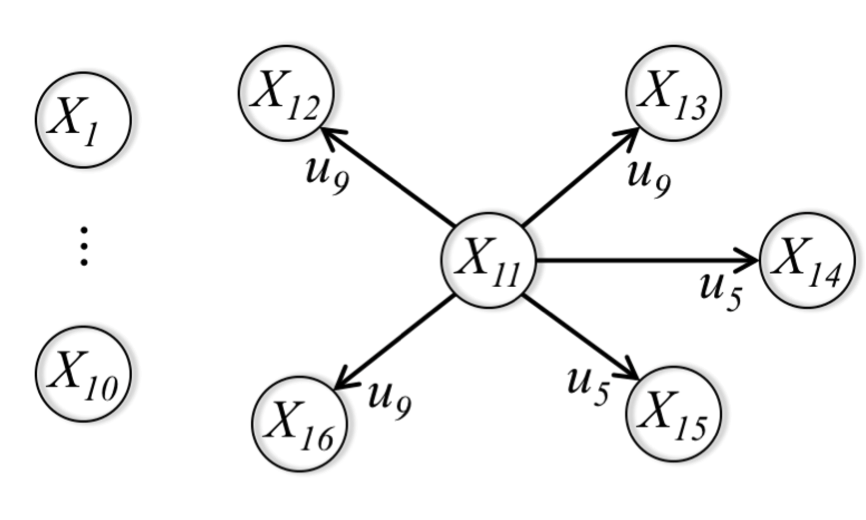
\includegraphics[width=0.3\textwidth]{exam2.png}
  \caption{An example of an AAF in situation $S_1$. Since $X_{11}$ defeats $X_{12}, X_{13}, X_{14}, X_{15}$ and $X_{16}$, the defeat relation between defeated arguments is omitted.}
    \label{fig:ex-2}
\end{figure}
\end{example}

%Note that for a new situation, the vectors of duty satisfaction/violation values are inherited from the identical trained situation (if it exists) in $SIT$. 

Third, given an AAF, 
the notion of argumentation semantics in \cite{DBLP:journals/ai/Dung95} can be used to evaluate the status of arguments. There are a number of argumentation semantics capturing different intuitions and constraints for evaluating the status of arguments in an AAF, including complete, preferred, grounded and stable, etc. First, a complete extension is defined in terms of the notions of conflict-freeness and defense. Given an AAF $(\mathcal{A}, \mathcal{R})$, we say that a subset $E\subseteq \mathcal{A}$ is conflict-free if and only if there exist no $X_1, X_2\in E$  such that $X_1$ defeats $X_2$; $E$ defends an argument $X\in \mathcal{A}$ if and only if for every argument $Y\in \mathcal{A}$ if $Y$ defeats $X$ then there exists $Z\in E$ such that $Z$ defeats $Y$. Set $E$ is admissible if and only if it is conflict-free and defends each argument in $E$. Then, we say that $E$ is a complete extension if and only if $E$ is admissible and each argument in $\mathcal{A}$ defended by $E$ is in $E$; $E$ is a preferred extension if and only if $E$ is a maximal complete extension with respect to set-inclusion; $E$ is the grounded extension if and only if $E$ is a minimal complete extension with respect to set-inclusion; $E$ is a stable extension if and only if $E$ defeats each argument in $\mathcal{A}\setminus E$. It has been verified that each AAF has a unique (possibly empty) set of grounded extension, while many AAFs may have multiple sets of extensions, which may be used to capture the intuition that there can be multiple solutions in some decision-making scenarios. When an AAF is acyclic, it has only one extension under all semantics. 
Then, we say that an argument of an AAF is skeptically justified under a given semantics if it is in every extension of the AAF, and credulously justified if it is in at least one but not all extensions of the AAF. For convenience, we use $\sigma$ to denote an argumentation semantics, which can be complete, grounded, stable or preferred. 
For more information about argumentation semantics, please refer to \cite{DBLP:journals/ker/BaroniCG11}.

\begin{example}[Argumentation semantics] \label{ex-argsem}
Consider the AF in Figure \ref{fig:ex-2}. It is acyclic and has only one extension under any argumentation semantics $\sigma$, i.e., $E = \{X_1, \dots, X_{10}, X_{11}\}$. In this example, all arguments in $E$ are skeptically justified.
\end{example}

Given a set of justified arguments, we may define the set of justified conclusions as follows. 

\begin{definition}[Justified conclusion]
Let $(\mathcal{A}, \mathcal{R})$ be an AAF, and $X\subseteq \mathcal{A}$ be a skeptically (credulously) justified argument under an argumentation semantics $\sigma$. A skeptically (credulously) justified conclusion is written as $concl(X)$. We say that $concl(X)$ is a skeptically (credulously) justified action if and only if $X$ is an action argument.
\end{definition}

\begin{example}[Justified conclusions] \label{ex-just}
According to Example \ref{ex-argsem}, all elements in $S_1\cup \{charge: v_{S_1}(charge)\}$ are justified conclusions, in which $charge: v_{S_1}(charge)$ or $charge$ is a justified action.
\end{example}

Now, let us verify that the representation by using argumentation-based approach is sound and complete under stable semantics. 

\begin{proposition}[Soundness and completeness of repre.]
Let $Ag = (\mathcal{L}, SIT, M, \pi)$ be a VDA, where $\mathcal{L} = (L, P$, $A, D)$. Let $\alpha\in A$ be an action. Given a situation $S\in SIT$ and an action matrix $M_S\in M$, it holds that $\alpha : v_{S}(\alpha)$ is a solution of $Ag$ with respect to $S$, if and only if $\alpha : v_{S}(\alpha)$ is a justified action in $F_{Ag, S} = (Arg(Ag, S), Def(Ag, S))$ under stable semantics.
\end{proposition}

\begin{proof}
On the one hand, if $\alpha : v_{S}(\alpha)$ is a  solution of $Ag$ with respect to $S$, then there exists an ordering over $A$, such that $\alpha$ is the first action of the sorted list. It follows that for each $\beta\in A \setminus \{\alpha\}$, either $v_{S}(\alpha) > v_{S}(\beta)$ or $\alpha$ and $\beta$ are not comparable. 
According to Definition \ref{def-arg}, there exist $X, Y\in Arg(Ag, S)$ such that $\alpha : v_{S}(\alpha) = concl(X)$ and $\beta : v_{S}(\beta) = concl(Y)$. It follows that $X$ defeats $Y$, or $X$ and $Y$ defeat each other. In either case, any argument defeating $X$ is defeated by $X$. It follows that $\{X\}\cup S$ is a stable extension. So, $\alpha : v_{S}(\alpha) = concl(X)$ is a justified action in $F_{Ag, S}$ under stable  semantics. 
On the other hand, if $\alpha : v_{S}(\alpha)$ is a justified action in $F_{Ag, S} = (Arg(Ag, S), Def(Ag, S))$ under stable semantics, then there exists $X\in Arg(Ag, S)$ such that $concl(X) = \alpha : v_{S}(\alpha)$. Since in situation $S$, any two different action arguments attack each other, no two action arguments can be in the same extension. So, $\{X\}\cup S$ is a stable extension of $F_{Ag, S}$. According to the definition of a stable extension, $X$ defeats each action argument in $Arg(Ag, S)\setminus \{X\}$. In other words, for every action argument $Y\in  Arg(Ag, S)\setminus \{X\}$ such that $concl(Y) = \beta: v_{S}(\beta)$, $v_{S}(\alpha) \ge_u v_{S}(\beta)$ for some $u\in\pi$. So, one may construct an ordering of actions such that $\alpha$ is the first action in the sorted list. Therefore, $\alpha : v_{S}(\alpha)$ is a solution of $Ag$ with respect to $S$.
\end{proof}

Based on arguments, defeat relation between arguments, and a set of justified conclusions, the explanation of choosing an action includes the following perspectives: state of the world (the premise of the accepted action argument), satisfied duty (in the conclusion of the accepted action argument), overturned actions and underlying reasons (the conclusions of defeated arguments, differentials of duty satisfaction/violation in the clause of a principle associated with each defeat). We use the following example to illustrate an explanation, while the formal definition is omitted. 

\begin{example}[Explanation]
According to Examples \ref{ex-2} and \ref{ex-just}, the explanation of the justified action $charge: v_{S_1}(charge)$ is as follows. 
\begin{description}
\item[] Action $charge$ is selected, because:
\begin{description}
\item[1.] Supporting argument $X_{11}$ is justified, with
\begin{description}
\item[-]perception battery low ($lb$) in the premise
\item[-]action $charge$ in the conclusion
\item[-]maximal duty satisfaction $\mathrm{MMR} = 2$ in $v_{S_1}(charge)$
\end{description}
\item[2.] All conflicting arguments are rejected, with action $charge$ more ethically preferable than
\begin{description}
\item[-] $remind$ in $X_{12}$ that is defeated by $X_{11}$ w.r.t. $u_9$
\item[-] $engage$ in $X_{13}$ that is defeated by $X_{11}$  w.r.t. $u_9$
\item[-] $warn$ in $X_{14}$ that is defeated by $X_{11}$  w.r.t. $u_5$
\item[-] $notify$ in $X_{15}$ that is defeated by $X_{11}$  w.r.t. $u_5$
\item[-] $seekTask$ in $X_{16}$ that is defeated by $X_{11}$  w.r.t. $u_9$
\end{description}
\end{description}
\end{description}
\end{example}


%The intuition of case supported principle-based behavior paradigm (CPB) is that a principle trained over time will correctly cover all cases of its domain. 

%\begin{proposition}
%Let $Ag = (\mathcal{L},  SIT, M, \pi)$ be a value driven agent, where $\mathcal{L} = (L, P, A, D)$. It holds that for every situation $S$, $sol(Ag, M_S, \pi) = concl(\sigma(F_{Ag, S}))$.
%\end{proposition}

%\begin{definition}
%Let $Ag = (\mathcal{L},  SIT, M, \pi)$ be a value driven agent and $E$ is extension of $F_{Ag, S}$. For every action-duty satisfaction/violation pair $\alpha: v \in concl(E)$, the explanation of $\alpha: v$ is a tuple $expl(\alpha: v) = (\mathrm{because}, \mathrm{promote}, \mathrm{overturn})$ 
%\end{definition}

%In current version of an explanation, we have not exploited the links between the clauses of a principle and the cases used to generate them. We leave this to future work.

\section{Discussion: Justification and explanation in more sophisticated autonomous agents}
In the previous two sections, we have introduced an argumentation-based formalism for representation, justification and explanation in a VDA. In the current version of VDA \cite{DBLP:journals/pieee/Anderson19}, we have not taken into consideration some more complicated scenarios. For instance, a VDA may not only have practical reasoning concerning which action should be selected, but also have epistemic reasoning about the state of the world. 
In this new scenario, besides a set perceptions, we may add epistemic rules, which could be strict or defeasible, to represent the knowledge of the world. 

\begin{definition}[Epistemic rule]
%There are two kinds of rules. 
Let $Ag = (\mathcal{L},  SIT, M, \pi)$ be a value driven agent, where $\mathcal{L} = (L, P, A, D)$. 
An epistemic rule of $Ag$ is either a strict rule $R: p_1, \dots, p_n \rightarrow  p$ or a defeasible rule $R: p_1, \dots, p_n \Rightarrow  p$, where  $p_i, p\in L$ are literals.  
\end{definition}

%The set of all action rules of a value driven agent  $Ag$ is denoted as $RULE(Ag)$. 

\begin{example}[Epistemic rule]\label{ex-ep-rules}
Assume that the message concerning whether the battery is low is obtained by observation. In this sense, the elements in $S_1$ are not all facts. Instead, they can be assumptions. For instance, now we consider $lb\in S_1$ as an assumption, denoting that the battery is presumably low by observation. Now, we assume that signal of battery is found abnormal ($ab$). In this case, we may infer that the battery is probably not low. We use a defeasible rule to represent this piece of knowledge: $R_7: ab \Rightarrow \neg lb$.
 
Due to incomplete and uncertain information, there may be several possible situations. According to Example \ref{ex-ep-rules}, there are two possible situations $S_1$ and $S_1^\prime = (S_1 \setminus \{lb\})\cup \{ab, \neg lb\}$. To justify which situation holds, one may construct an AAF at the epistemic level, visualized in the left part of Figure \ref{fig:ex-21}, in which two additional arguments are as follows. We assume that $R_{18}$ is superior to the assumption $lb$.
\begin{description}
\item[]$X_{17}$ : $ab$
\item[]$X_{18}$: $X_{17} \Rightarrow \neg lb$
\end{description}

By using the AAF in left part of Figure \ref{fig:ex-21}, we may justify that $S_1^\prime$ holds. Under this situation, the action matrix is as follows.

\begin{description}
\item $v_{S_1}(charge) = (0, 1,  0, -1, 0, 0, 0)$.
\item $v_{S_1}(remind) = (-1, -1, 0, -1, 0, 0, 0)$.
\item $v_{S_1}(engage) = (0, -1, 0, -1, 0, 0, 0)$.
\item $v_{S_1}(warn) = (0, 0, 0, -1, 0, -1, 0)$.
\item $v_{S_1}(notify) = (0, 0, 0, -1, 0, -2, 0)$.
\item $v_{S_1}(seekTask) = (0, -1, 0, 1, 0, 0, 0)$.
\end{description}

Similar to the previous examples, an AAF for practical reasoning under situation $S^\prime_1$ is visualized in the right part of Figure \ref{fig:ex-21}. Similarly, defeat relation between defeated arguments is omitted.

\begin{figure}[h!]
  \centering
 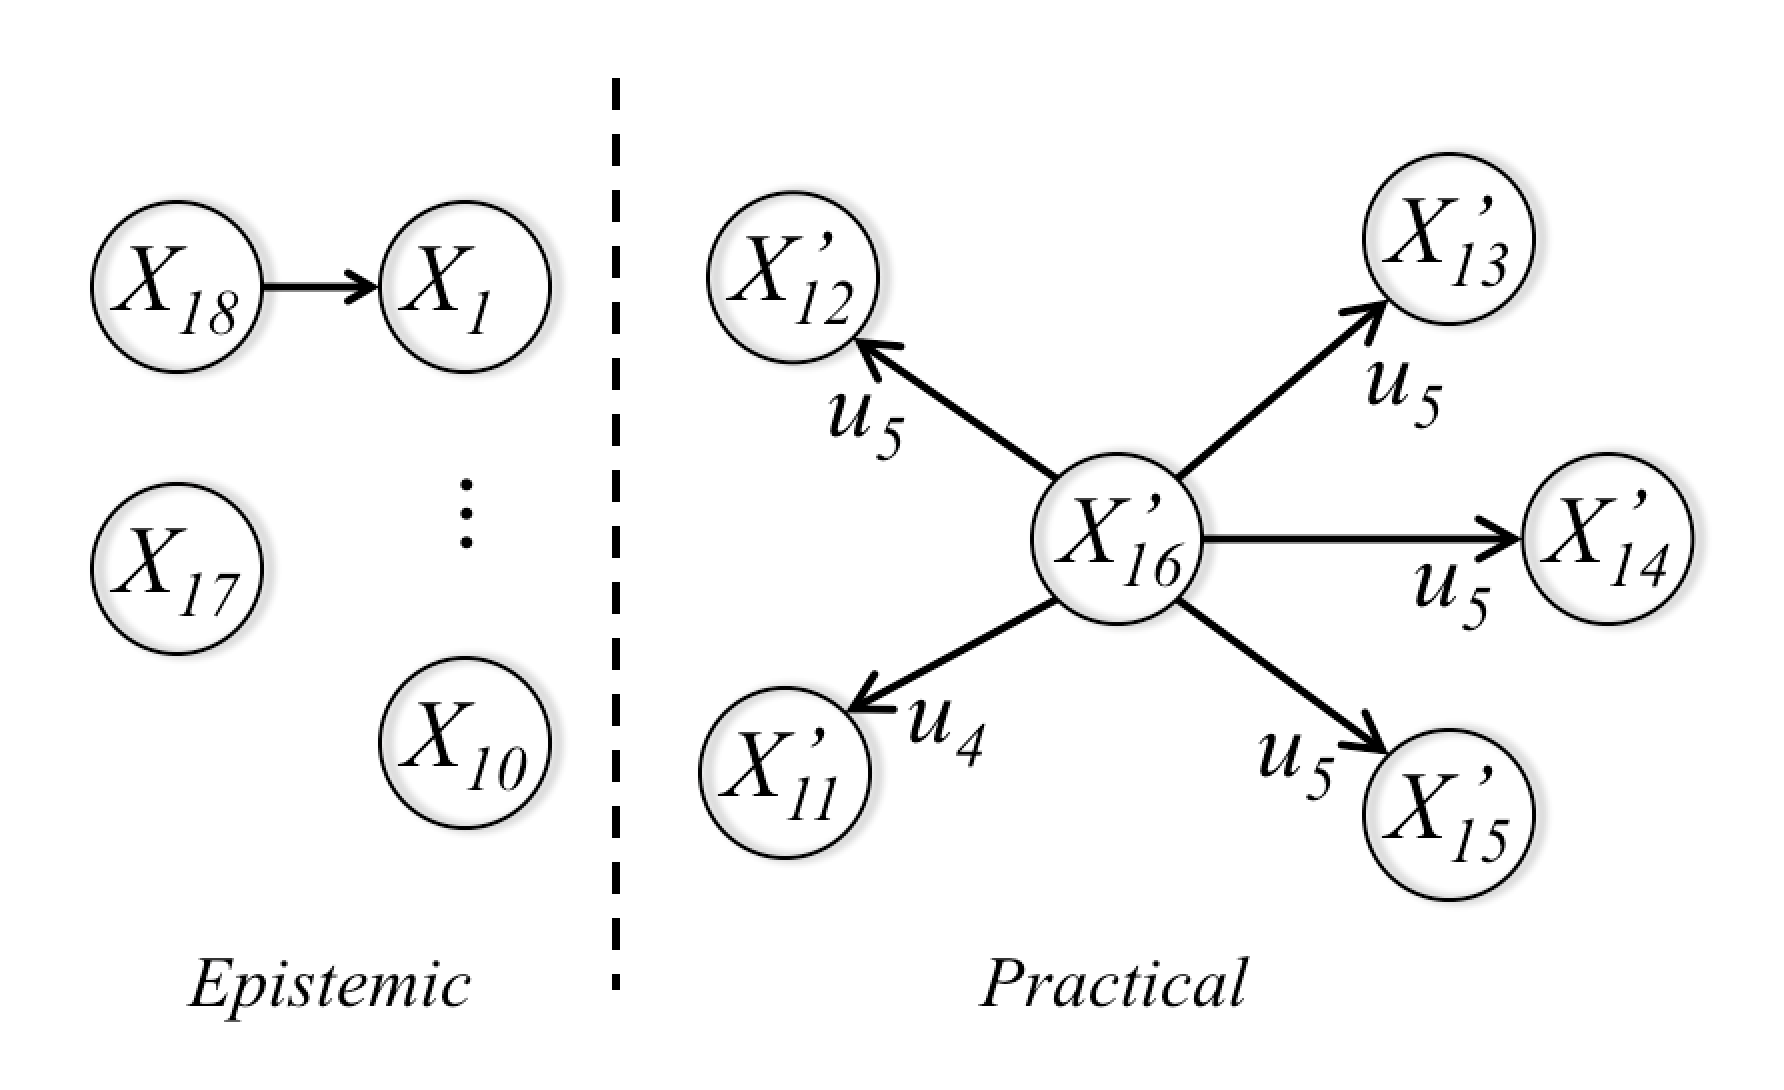
\includegraphics[width=0.38\textwidth]{exam5.png}
  \caption{AAFs for epistemic and practical reasoning}
    \label{fig:ex-21}
\end{figure}
\end{example}

In this updated scenario, the justified action is $seekTask$ that is supported by the justified argument $X^\prime_{16}$. Now, let us present an updated explanation for the new justified action. 

\begin{example}[Updated explanation]
The explanation of the justified action $seekTask$ is as follows. 
\begin{description}
\item[] Action $seekTask$ is selected, because:
\begin{description}
\item[1.] Argument $X_{18}$ supporting situation $S_1^\prime$ is justified, with $\neg lb$ in the conclusion of $X_{18}$.
\item[2.] Supporting argument $X_{16}^\prime$ is justified, with
 battery not low ($\neg lb$) in the premise,
 action $seekTask$ in the conclusion, and
 maximal duty satisfaction $\mathrm{MG2P} = 1$ in the conclusion.
\item[3.] All conflicting action arguments are rejected, with action $seekTask$ more ethically preferable than
\begin{description}
\item[-]  $charge$ in $X_{11}^\prime$ that is defeated by $X_{16}^\prime$ w.r.t. $u_4$ 
\item[-]  $remind$ in $X_{12}^\prime$ that is defeated by $X_{16}^\prime$ w.r.t. $u_5$ 
\item[-]  $engage$ in $X_{13}^\prime$ that is defeated by $X_{16}^\prime$ w.r.t. $u_5$ 
\item[-]  $warn$ in $X_{14}^\prime$ that is defeated by $X_{16}^\prime$ w.r.t. $u_5$ 
\item[-]  $notify$ in $X_{15}^\prime$ that is defeated by $X_{16}^\prime$ w.r.t. $u_5$ 
\end{description}
\end{description}
\end{description}
\end{example}

From the above examples, we may observe that for more sophisticated autonomous agents, there may be more than one type of reasoning, and different components of a system may be entangled. One example in this direction is the BOID architecture introduced in   \cite{DBLP:conf/agents/BroersenDHHT01}. Furthermore, in a multi-agent system, reasoning about actions of one agent is dependent both on the individual values of the agent concerned and on what others choose to do \cite{DBLP:journals/ai/AtkinsonB18}. 

%In our existing version of VDA \cite{DBLP:journals/pieee/Anderson19}, neither espitemic reasoning nor multi-agent interaction has been considered. We leave such extensions to the VDA for future work.



\section{Conclusions}
In this paper, we have proposed an argumentation-based approach for representation, justification and explanation of a VDA. The contributions are three-fold. First, we provide a formalism to represent a VDA, making explicit some implicit knowledge. This lays a foundation for the justification and explanation of reasoning and decision making in a VDA. Second, we adapt existing structured and abstract argumentation theories to the setting of a decision making in a VDA, such that the priority relation and defeat relation over arguments are linked to the ethical consequences of actions that are reflected by clauses of a principle, and the justification and explanation of an action can be defined accordingly. Third, unlike existing argumentation systems where formal rules are designed in advance, in our approach, rules are generated and updated at run time by automatically translating a situation and an action matrix to a set of rules, while the priority relation between rules is also dynamically evaluated in terms of a principle. Thanks to the graphic nature of an AAF, when the system becomes more complex, there exist efficient approaches to handle the dynamics of the system, e.g., \cite{DBLP:journals/ai/LiaoJK11,DBLP:books/daglib/0033440}.

Concerning future work, first, we have not identified nor formally represented the relation between a principle and a set of cases from which the principle is learned. Doing so is likely to provide further information that explains why an action is chosen in a given situation. Second, in the existing version of VDA \cite{DBLP:journals/pieee/Anderson19}, neither espitemic reasoning nor multi-agent interaction \cite{DBLP:conf/agents/BroersenDHHT01,DBLP:journals/ai/AtkinsonB18,handbooknms} has been considered. The addition of such extensions to the VDA will serve to extend its capabilities.

The work reported in this paper shares some similarity with the symbolic approach introduced in \cite{DBLP:conf/ijcai/ShihCD18}, in the sense that some implicit functions of the system is made explicit by using a symbolic representation. However, rather than translating the function between a set of features and a classification, we translate several types of implicit knowledge of a VDA by a logical formalism. Other related works are those based on argumentation, e.g., \cite{Cocarascu2018}, in which an AAF is constructed in terms of highest ranked features. To the best of our knowledge, no work in existing literature exploits argumentation to address similar research problems in the present paper. 

Clearly, formal justification and explanation of the behavior of autonomous systems enhances the transparency of such systems.  Further, we contend that autonomous systems that can argue formally for their actions are more likely to engender trust in their users than systems without such a capability. That principle-based systems such as the one detailed in this paper and others (e.g. \cite{VANDERELST201856,sarathyetal2017coginfocom}) seem to lend themselves readily to explanatory mechanisms adds further support for their adoption as a formalism to ensure the ethical behavior of autonomous systems. 



%Background: self-driving cars, AI medical, heath care, etc.  

%Trust and explanations in AI systems. 

%How an agent's actions can be aligned with human values?   A short review of papers about value alignment.  Anderson \& Anderson's work:  learning human (ethicists)'s values through inductive learning, and obtaining principles that define a partial order on actions. The principles may change under different contexts, cultural, legal, etc (Blass 2018).  However, there is no explicit representation of norms, and lack of explanation in terms of this explicit representation of  knowledge. 

%(Blass \& Horswill, 2015) uses defeasible logic to model ethical norms. 

%ethical dilemmas refer to cases in which any available choice leads to infringing some accepted ethical principles and yet a decision has to be made [Kirkpatrick, 2015]. 

%So, for each action, a set of values promoted or demoted is attached.  

%generalized frameworks are preferred over ad-hoc rules.

%ethical bounds can be contextual and difficult to define as  design time

%the ethically correct actions that a robot should perform will be domain dependent. 


%individual ethical decision framework: 


%Joseph A. Blass. Legal, Ethical, Customizable Artificial Intelligence. AIES2018. 

%Blass, J.A. and Horswill, I. 2015. Implementing Injunctive Social
%Norms using Defeasible Reasoning. Workshop on Social Believability,
%Procs of the Eleventh AAAI Conference on Artificial Intelligence
%and Interactive Digital Entertainment. Santa Cruz, CA.




%\section{Conclusions}
%In this paper, we have formulated ... 


%\section*{Acknowledgments}
% The research reported in this paper was partially supported by the National
%Research Fund Luxembourg (FNR) under grant INTER/MOBILITY/14/8813732
%for the project FMUAT: Formal Models for Uncertain Argumentation from Text,
%and the European Union's Horizon 2020 research and innovation programme
%under the Marie Sklodowska-Curie grant agreement No 690974 for the project
%MIREL: MIning and REasoning with Legal texts.  Further support has been provided by the United States National Science Foundation under Grant Numbers IIS-0500133, IIS-1151305 and IIS-1449155.  
 
 
\bibliographystyle{aaai}
\bibliography{AIEs2019}

\end{document}
